\title[Position, Velocity, and Acceleration]{Position, Velocity, and Acceleration}
\subtitle{Physics I · Mechanics Practice Session · \labversionlabel}
\author{}
\institute{}
\date{Week 1}

\begin{document}

\begin{frame}[plain]
  \begin{tikzpicture}[remember picture,overlay]
    \node[anchor=north west,inner sep=0pt] at (current page.north west) {
      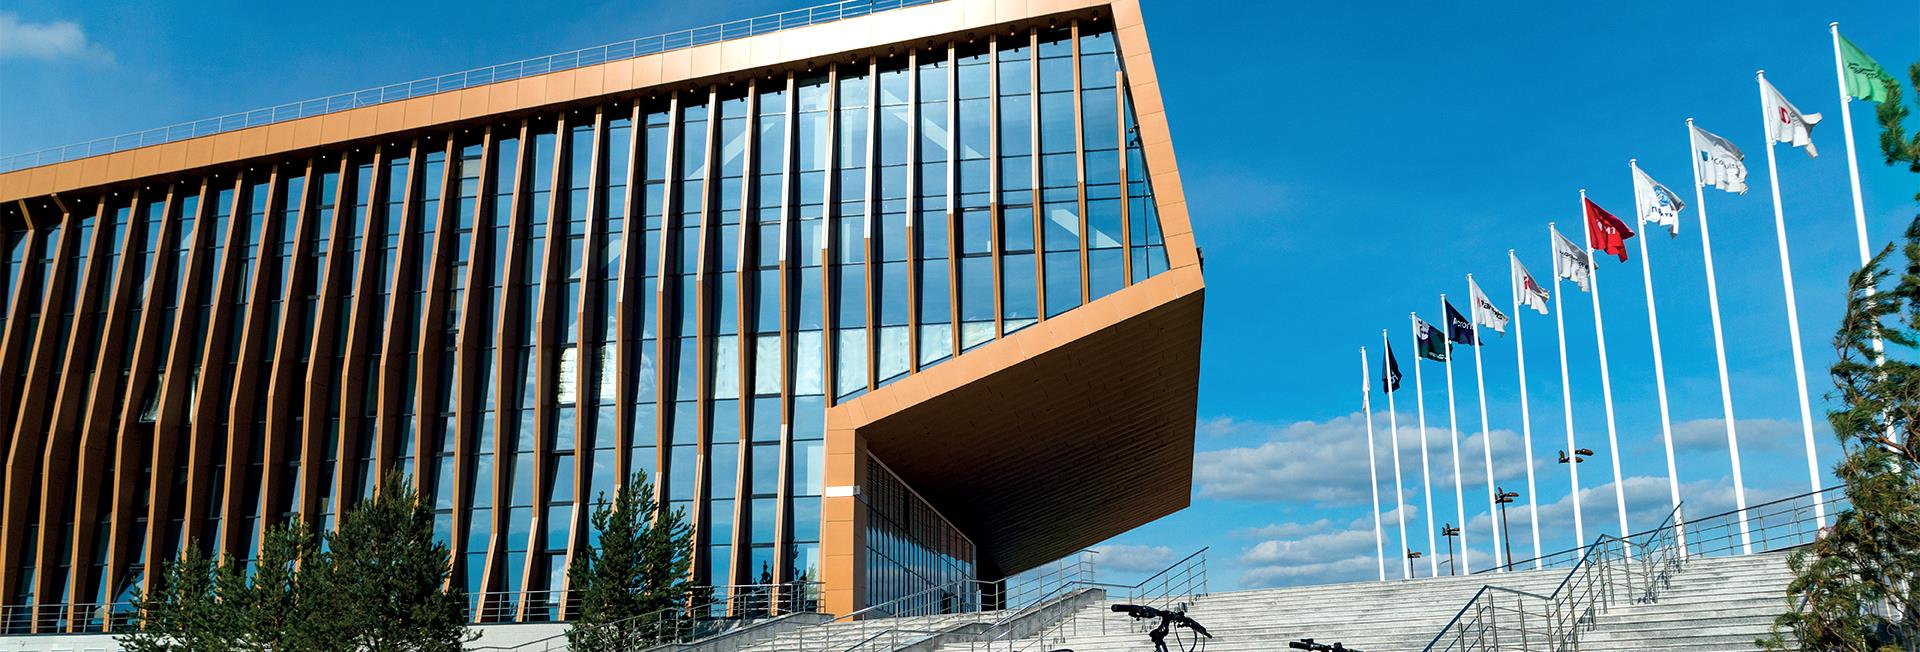
\includegraphics[width=\paperwidth,height=0.58\paperheight]
        {assets/innopolis-campus.jpg}%
    };
    \fill[white]
      (current page.south west) rectangle
      ([yshift=-0.58\paperheight]current page.north east);
    \fill[PhysicsBlue]
      (current page.south west) rectangle
      ([xshift=0.012\paperwidth,yshift=-0.58\paperheight]current page.north west);
    \node[anchor=north west,text width=0.86\paperwidth,align=left]
      at ([xshift=0.055\paperwidth,yshift=-0.64\paperheight]current page.north west) {
        {\color{PhysicsBlue}\small\bfseries PHYSICS I · MECHANICS PRACTICE SESSION\par}
        \vspace{0.45em}
        {\color{PhysicsInk}\fontsize{17}{20}\selectfont\bfseries
          Position, Velocity, and Acceleration\par}
        \vspace{0.55em}
        {\color{PhysicsMuted}\small Week 1 · \labversionlabel\par}
      };
    \node[anchor=east,inner sep=0pt]
      at ([xshift=-0.055\paperwidth,yshift=0.16\paperheight]current page.south east) {
        
\includegraphics[width=0.20\paperwidth]
          {assets/innopolis-university-logo.png}%
      };
  \end{tikzpicture}
\end{frame}

\begin{frame}{Brief Review: One-Dimensional Motion}
  \begin{columns}[T,onlytextwidth]
    \begin{column}{0.48\textwidth}
      \begin{block}{Average velocity and acceleration}
        \[
          \bar v=\frac{\Delta x}{\Delta t},
          \qquad
          \bar a=\frac{\Delta v}{\Delta t}
        \]
      \end{block}
      \begin{block}{Instantaneous velocity and acceleration}
        \[
          v=\frac{\mathrm{d}x}{\mathrm{d}t},
          \qquad
          a=\frac{\mathrm{d}v}{\mathrm{d}t}
        \]
      \end{block}
    \end{column}
    \begin{column}{0.48\textwidth}
      \begin{block}{Distance covered in one-directional motion}
        \[
          S=\int v(t)\,\mathrm{d}t
        \]
      \end{block}
      \footnotesize
      \textbf{Symbols:}
      $x$ — position; $S$ — distance; $t$ — time;
      $v$ — velocity; $a$ — acceleration;
      $\Delta$ — change in a quantity.
    \end{column}
  \end{columns}
  \vspace{0.35em}
  \begin{beamercolorbox}[rounded=true,sep=0.55em,wd=\linewidth]{block body}
    \footnotesize
    \textbf{Units:}
    \texttt{m} — metre; \texttt{km} — kilometre;
    \texttt{cm} — centimetre; \texttt{s} — second; \texttt{h} — hour;
    \texttt{m/s} — metres per second;
    \texttt{m/s\textsuperscript{2}} — metres per second squared;
    \texttt{m/s\textsuperscript{3}} — metres per second cubed;
    \texttt{km/h} — kilometres per hour;
    \texttt{cm/s} — centimetres per second.
  \end{beamercolorbox}
\end{frame}

\begin{frame}{Position and Velocity from Integration}
  \small
  \begin{columns}[T,onlytextwidth]
    \begin{column}{0.62\textwidth}
      \begin{align*}
        x(T)&=x_i+\int_0^T v(t)\,\mathrm{d}t,\\
        v(T)&=v_i+\int_0^T a(t)\,\mathrm{d}t,\\
        x(T)&=x_i+v_iT+\int_0^T\!\mathrm{d}t
          \int_0^t a(h)\,\mathrm{d}h.
      \end{align*}
    \end{column}
    \begin{column}{0.34\textwidth}
      \begin{block}{Notation}
        \footnotesize
        $x_i$ — initial position

        $v_i$ — initial velocity

        $T$ — current time

        $t,h$ — time variables

        $a(t)$ — arbitrary acceleration
      \end{block}
    \end{column}
  \end{columns}
  \vspace{0.35em}
  \begin{block}{For constant acceleration $a$}
    \[
      x(T)=x_i+v_iT+\frac{aT^2}{2}
    \]
  \end{block}
\end{frame}

\begin{frame}{Problem 1 — Trains and a Bird}
  \slidetag{PROBLEM 1}
  \vspace{0.15em}
  \scriptsize
  Model the two trains as \textbf{black material points (black MPs)}, each
  moving at $V_b=\SI{30}{\kilo\metre\per\hour}$, and the bird as a
  \textbf{white material point (white MP)} moving at
  $V_w=\SI{60}{\kilo\metre\per\hour}$. The black MPs approach each other on
  the same straight track. When they are \SI{60}{\kilo\metre} apart, the white
  MP starts at one black MP and moves back and forth between them until they
  collide.
  \vspace{0.2em}
  \begin{block}{Find}
    What total distance does the white MP travel before the black MPs collide?
  \end{block}
  \vspace{-0.2em}
  \centering
  \resizebox{0.76\textwidth}{!}{\begin{tikzpicture}[
  x=1cm,
  y=1cm,
  black mp/.style={circle,fill=PhysicsInk,draw=PhysicsInk,minimum size=5.5pt,
    inner sep=0pt},
  white mp/.style={circle,fill=white,draw=PhysicsInk,line width=0.8pt,
    minimum size=5.5pt,inner sep=0pt},
  motion/.style={-{Latex[length=2.2mm]},PhysicsInk,line width=0.9pt},
  track/.style={PhysicsInk,line width=0.9pt}
]
  % Legend: the names used in the professor's material-point model.
  \node[black mp] at (4.05,5.05) {};
  \node[anchor=west,font=\scriptsize\sffamily] at (4.18,5.05)
    {black MP (train)};
  \node[white mp] at (7.0,5.05) {};
  \node[anchor=west,font=\scriptsize\sffamily] at (7.13,5.05)
    {white MP (bird)};

  % Time runs downward, as in the source schematic.
  \draw[-{Latex[length=2.8mm]},PhysicsInk,line width=1pt]
    (0.45,4.65) -- (0.45,0.15);
  \node[rotate=90,font=\small\sffamily] at (0.12,2.4)
    {Evolution of the system, time};

  % Initial state.
  \draw[track] (1.15,4.25) -- (10.75,4.25);
  \node[black mp] at (2.05,4.25) {};
  \node[white mp] at (2.30,4.25) {};
  \node[black mp] at (9.85,4.25) {};
  \draw[physics dimension] (2.05,3.88) --
    node[below,font=\scriptsize\sffamily] {$S=\SI{60}{\kilo\metre}$}
    (9.85,3.88);
  \node[anchor=west,font=\scriptsize\sffamily] at (10.9,4.25)
    {initial position};

  % First flight of the white material point.
  \draw[track] (1.15,2.95) -- (10.75,2.95);
  \node[black mp] at (2.95,2.95) {};
  \node[white mp] at (5.2,2.95) {};
  \node[black mp] at (9.0,2.95) {};
  \draw[motion] (3.05,3.15) -- node[above,font=\scriptsize\sffamily] {$V_b$}
    (3.75,3.15);
  \draw[motion] (5.3,3.15) -- node[above,font=\scriptsize\sffamily] {$V_w$}
    (6.2,3.15);
  \draw[motion] (8.9,3.15) -- node[above,font=\scriptsize\sffamily] {$-V_b$}
    (8.2,3.15);

  % Return flight after the trains have moved closer.
  \draw[track] (1.15,1.72) -- (10.75,1.72);
  \node[black mp] at (3.55,1.72) {};
  \node[white mp] at (6.7,1.72) {};
  \node[black mp] at (8.35,1.72) {};
  \draw[motion] (3.65,1.92) -- node[above,font=\scriptsize\sffamily] {$V_b$}
    (4.35,1.92);
  \draw[motion] (6.6,1.92) -- node[above,font=\scriptsize\sffamily] {$-V_w$}
    (5.7,1.92);
  \draw[motion] (8.25,1.92) -- node[above,font=\scriptsize\sffamily] {$-V_b$}
    (7.55,1.92);

  % Final state.
  \draw[track] (1.15,0.55) -- (10.75,0.55);
  \node[black mp] at (5.82,0.55) {};
  \node[white mp] at (6.02,0.55) {};
  \node[black mp] at (6.22,0.55) {};
  \node[below=3pt,font=\scriptsize\sffamily] at (6.02,0.55) {collision};
  \node[anchor=west,font=\scriptsize\sffamily] at (10.9,0.55)
    {final position};
\end{tikzpicture}
}
\end{frame}

\begin{solutionframe}[Solution 1 — Collision Time]
  \footnotesize
  Let $S$ be the initial separation. Because the black MPs have opposite
  velocities, their closing speed is
  \[
    V_{\mathrm{close}}=V_b-(-V_b)=2V_b.
  \]
  The collision time and the distance traveled by the white MP are therefore
  \[
    t_c=\frac{S}{V_{\mathrm{close}}}=\frac{S}{2V_b},
    \qquad
    S_w=V_wt_c=\frac{V_wS}{2V_b}.
  \]
  \begin{block}{Why the repeated flights need not be added separately}
    Every flight occurs during the same total interval $t_c$; only the white
    MP's constant speed and the collision time are needed.
  \end{block}
  \answer{\(\displaystyle
    t_c=\frac{\SI{60}{\kilo\metre}}
      {2(\SI{30}{\kilo\metre\per\hour})}=\SI{1}{\hour},\qquad
    S_w=(\SI{60}{\kilo\metre\per\hour})(\SI{1}{\hour})
      =\SI{60}{\kilo\metre}\)}
\end{solutionframe}

\begin{frame}{Problem 2(a) — Cheetah Pursuit}
  \slidetag{PROBLEM 2A}
  \vspace{0.35em}
  \begin{columns}[T,onlytextwidth]
    \begin{column}{0.54\textwidth}
      \small
      A cheetah can run at about
      \SI{101}{\kilo\metre\per\hour} for perhaps \SI{20}{\second}. An
      antelope can run at about \SI{88}{\kilo\metre\per\hour} for much
      longer. Both animals run in the same direction at top speed, and the
      antelope has a \SI{40}{\metre} head start.
      \vspace{0.55em}
      \begin{block}{Find}
        How long does the cheetah take to catch the antelope, and how far does
        the cheetah travel in that time?
      \end{block}
    \end{column}
    \begin{column}{0.42\textwidth}
      \centering
      \begingroup
        \def\cheetahparta{1}
        \resizebox{\textwidth}{!}{\begin{tikzpicture}[
  x=1cm,
  y=0.85cm,
  axis arrow/.style={-{Latex[length=2.5mm]},PhysicsNavy,line width=1pt}
]
  \draw[axis arrow] (0,0) -- (7.2,0) node[right,font=\small\sffamily] {$t$};
  \draw[axis arrow] (0,0) -- (0,5.8) node[above,font=\small\sffamily] {$x$};
  \draw[PhysicsRed,line width=1.5pt] (0,0) -- (6,5);
  \draw[PhysicsBlue,line width=1.5pt] (0,1.3) -- (6,5);
  \fill[PhysicsNavy] (6,5) circle[radius=2.8pt];
  \node[above left,font=\small\sffamily] at (6,5) {capture};
  \node[rotate=39,font=\scriptsize\sffamily,text=PhysicsRed,
    fill=white,inner sep=1pt] at (3.6,3.0)
    {cheetah: \SI{101}{\kilo\metre\per\hour}};
  \node[rotate=31,font=\scriptsize\sffamily,text=PhysicsBlue,
    fill=white,inner sep=1pt] at (3.7,3.7)
    {antelope: \SI{88}{\kilo\metre\per\hour}};

  \ifdefined\cheetahparta
    \draw[physics dimension] (-0.45,0.05) --
      node[left,font=\scriptsize\sffamily,align=right] {head start\\\SI{40}{\metre}}
      (-0.45,1.25);
    \draw[PhysicsMuted,dashed] (6,0) -- (6,4.85);
    \node[below,font=\scriptsize\sffamily,text=PhysicsMuted] at (6,0) {$t=?$};
  \fi

  \ifdefined\cheetahpartb
    \draw[physics dimension] (-0.45,0.05) --
      node[left,font=\scriptsize\sffamily,align=right] {head start\\$?$}
      (-0.45,1.25);
    \draw[PhysicsMuted,dashed] (6,0) -- (6,4.85);
    \node[below,font=\scriptsize\sffamily,text=PhysicsMuted] at (6,0)
      {$t=\SI{20}{\second}$};
  \fi
\end{tikzpicture}
}
      \endgroup
    \end{column}
  \end{columns}
\end{frame}

\begin{solutionframe}[Solution 2(a) — Catch Time and Distance]
  \footnotesize
  Let $h$ be the antelope's head start. Choose $x_C(0)=0$ for the cheetah:
  \[
    x_C(t)=v_Ct,
    \qquad
    x_A(t)=h+v_At.
  \]
  At capture, $x_C=x_A$. Solve before inserting the data:
  \[
    \begin{aligned}
      v_Ct&=h+v_At,\\
      (v_C-v_A)t&=h,\\
      t_c&=\frac{h}{v_C-v_A},
      \qquad
      x_C(t_c)=\frac{v_Ch}{v_C-v_A}.
    \end{aligned}
  \]
  \answer{\scriptsize\(\begin{aligned}
    v_C&=101/3.6=\SI{28.06}{\metre\per\second},&
    v_A&=88/3.6=\SI{24.44}{\metre\per\second},\\
    v_C-v_A&=\frac{101-88}{3.6}
      =\SI{3.611}{\metre\per\second},\\
    t_c&=\frac{\SI{40}{\metre}}
      {(13/3.6)\,\si{\metre\per\second}}
      =\SI{11.08}{\second},&
    x_C&=\frac{(101/3.6)(40)}{13/3.6}\,\si{\metre}
      \approx\SI{310.8}{\metre}.
  \end{aligned}\)}
  \teacheronly{The professor's answer slide gives the time but not the second
    requested quantity. The distance follows directly from the stated data.}
\end{solutionframe}

\begin{frame}{Problem 2(b) — Maximum Head Start}
  \slidetag{PROBLEM 2B}
  \vspace{0.35em}
  \begin{columns}[T,onlytextwidth]
    \begin{column}{0.53\textwidth}
      \small
      Use the same top speeds:
      \[
        v_C=\SI{101}{\kilo\metre\per\hour},
        \qquad
        v_A=\SI{88}{\kilo\metre\per\hour}.
      \]
      The cheetah can maintain its maximum speed for only about
      \SI{20}{\second}.
      \vspace{0.55em}
      \begin{block}{Find}
        What is the maximum head start the antelope can have if the cheetah is
        to catch it within \SI{20}{\second}?
      \end{block}
    \end{column}
    \begin{column}{0.43\textwidth}
      \centering
      \begingroup
        \def\cheetahpartb{1}
        \resizebox{\textwidth}{!}{\begin{tikzpicture}[
  x=1cm,
  y=0.85cm,
  axis arrow/.style={-{Latex[length=2.5mm]},PhysicsNavy,line width=1pt}
]
  \draw[axis arrow] (0,0) -- (7.2,0) node[right,font=\small\sffamily] {$t$};
  \draw[axis arrow] (0,0) -- (0,5.8) node[above,font=\small\sffamily] {$x$};
  \draw[PhysicsRed,line width=1.5pt] (0,0) -- (6,5);
  \draw[PhysicsBlue,line width=1.5pt] (0,1.3) -- (6,5);
  \fill[PhysicsNavy] (6,5) circle[radius=2.8pt];
  \node[above left,font=\small\sffamily] at (6,5) {capture};
  \node[rotate=39,font=\scriptsize\sffamily,text=PhysicsRed,
    fill=white,inner sep=1pt] at (3.6,3.0)
    {cheetah: \SI{101}{\kilo\metre\per\hour}};
  \node[rotate=31,font=\scriptsize\sffamily,text=PhysicsBlue,
    fill=white,inner sep=1pt] at (3.7,3.7)
    {antelope: \SI{88}{\kilo\metre\per\hour}};

  \ifdefined\cheetahparta
    \draw[physics dimension] (-0.45,0.05) --
      node[left,font=\scriptsize\sffamily,align=right] {head start\\\SI{40}{\metre}}
      (-0.45,1.25);
    \draw[PhysicsMuted,dashed] (6,0) -- (6,4.85);
    \node[below,font=\scriptsize\sffamily,text=PhysicsMuted] at (6,0) {$t=?$};
  \fi

  \ifdefined\cheetahpartb
    \draw[physics dimension] (-0.45,0.05) --
      node[left,font=\scriptsize\sffamily,align=right] {head start\\$?$}
      (-0.45,1.25);
    \draw[PhysicsMuted,dashed] (6,0) -- (6,4.85);
    \node[below,font=\scriptsize\sffamily,text=PhysicsMuted] at (6,0)
      {$t=\SI{20}{\second}$};
  \fi
\end{tikzpicture}
}
      \endgroup
    \end{column}
  \end{columns}
\end{frame}

\begin{solutionframe}[Solution 2(b) — Maximum Head Start]
  Let $T$ be the maximum time for which the cheetah can maintain its top
  speed. From part (a),
  \[
    t_c=\frac{h}{v_C-v_A}.
  \]
  The largest possible head start corresponds to $t_c=T$:
  \[
    T=\frac{h_{\max}}{v_C-v_A},
    \qquad
    h_{\max}=(v_C-v_A)T.
  \]
  \answer{\(\begin{aligned}
    v_C-v_A&=\frac{101-88}{3.6}
      =\SI{3.61}{\metre\per\second},\\
    h_{\max}&=(\SI{3.61}{\metre\per\second})(\SI{20}{\second})
      =\SI{72.2}{\metre}\approx\SI{72}{\metre}.
  \end{aligned}\)}
\end{solutionframe}

\begin{frame}{Problem 3 — Police Pursuit}
  \slidetag{PROBLEM 3}
  \vspace{0.2em}
  \footnotesize
  A motorist traveling at \SI{31}{\metre\per\second} passes a stationary
  motorcycle police officer. \SI{2.5}{\second} later, the officer starts to
  move with constant acceleration
  \SI{3.6}{\metre\per\second\squared} in pursuit.
  \begin{block}{Find}
    How fast is the officer traveling when the motorcycle overtakes the car?
    Draw $x(t)$ for both objects, taking $t=0$ when the car passes the
    stationary officer.
  \end{block}
  \centering
  \resizebox{0.74\textwidth}{!}{\begin{tikzpicture}[x=1cm,y=1cm]
  \draw[PhysicsInk,line width=1.2pt] (0.15,0.35) -- (10.15,0.35);

  \node[anchor=south] at (2.1,0.4)
    {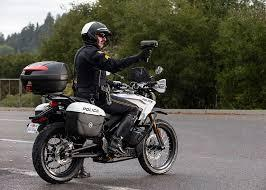
\includegraphics[width=3.0cm,height=2.0cm,keepaspectratio]{assets/problem3-motorcycle.png}};
  \node[anchor=south] at (7.55,0.4)
    {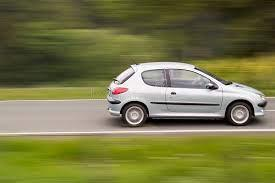
\includegraphics[width=3.1cm,height=2.0cm,keepaspectratio]{assets/problem3-car.png}};

  \node[font=\small\sffamily] at (2.1,2.72) {$v_m=0$};
  \node[font=\small\sffamily] at (7.55,2.72)
    {$v_c=\SI{31}{\metre\per\second}$};

  \draw[{Latex[length=2.2mm]}-{Latex[length=2.2mm]},PhysicsInk,line width=0.9pt]
    (3.7,1.35) -- node[above=3pt,font=\small\sffamily]
    {$t=\SI{2.5}{\second}$} (5.95,1.35);
  \draw[-{Latex[length=2.5mm]},PhysicsInk,line width=1pt]
    (9.2,1.35) -- (10.15,1.35);

  \node[font=\small\sffamily] at (2.1,0.03) {$x_m$};
  \node[font=\small\sffamily] at (7.55,0.03) {$x_c$};
\end{tikzpicture}
}
\end{frame}

\begin{solutionframe}[Solution 3 — Motion Laws]
  Set $x=0$ at the officer and $t=0$ when the car passes. The car moves at
  constant velocity:
  \[
    x_c(t)=v_ct.
  \]
  Let $t_d$ be the delay and $a_m$ the motorcycle's constant acceleration. The
  motorcycle is stationary until $t_d$, then starts from rest:
  \[
    x_m(t)=
    \begin{cases}
      0, & 0\le t<t_d,\\[2pt]
      \dfrac12a_m(t-t_d)^2, & t\ge t_d.
    \end{cases}
  \]
  These equations are now ready for the event condition $x_m=x_c$.
\end{solutionframe}

\begin{solutionframe}[Solution 3 — Overtaking Time]
  \footnotesize
  \setlength{\abovedisplayskip}{3pt}
  \setlength{\belowdisplayskip}{3pt}
  At the overtake, $x_m=x_c$:
  \[
    \begin{aligned}
      \frac12a_m(t-t_d)^2&=v_ct,\\
      a_mt^2-2(a_mt_d+v_c)t+a_mt_d^2&=0.
    \end{aligned}
  \]
  The quadratic formula gives
  \[
    t_{1,2}=\frac{a_mt_d+v_c
      \mp\sqrt{v_c^2+2a_mt_dv_c}}{a_m}.
  \]
  Only a root satisfying $t\ge t_d$ belongs to the motorcycle's moving branch.
  \answer{\scriptsize\(\begin{aligned}
    3.6t^2-2\!\left[3.6(2.5)+31\right]t+3.6(2.5)^2&=0,\\
    3.6t^2-80t+22.5&=0,\\
    t_{1,2}&=\frac{80\mp\sqrt{80^2-4(3.6)(22.5)}}{2(3.6)},\\
    t_1&=\SI{0.28}{\second}<t_d\ \text{(reject)},\qquad
    t_2=\SI{21.9}{\second}>t_d\ \text{(overtake)}.
  \end{aligned}\)}
\end{solutionframe}

\begin{solutionframe}[Solution 3 — Position–Time Curves]
  \centering
  \resizebox{0.78\textwidth}{!}{\begin{tikzpicture}
  \begin{axis}[
    width=11.3cm,
    height=5.7cm,
    axis lines=left,
    axis line style={PhysicsNavy,-{Latex[length=2.2mm]}},
    xmin=0,xmax=23,
    ymin=0,ymax=740,
    xlabel={$t$ (\si{\second})},
    ylabel={$x$ (\si{\metre})},
    tick label style={font=\scriptsize\sffamily},
    label style={font=\small\sffamily},
    grid=major,
    grid style={PhysicsLine},
    legend style={at={(0.03,0.97)},anchor=north west,draw=none,
      fill=white,font=\scriptsize\sffamily}
  ]
    \addplot[PhysicsBlue,line width=1.5pt,domain=0:22.5,samples=2] {31*x};
    \addlegendentry{car: $x_c=31t$}
    \addplot[PhysicsRed,line width=1.5pt] coordinates {(0,0) (2.5,0)};
    \addplot[PhysicsRed,line width=1.5pt,domain=2.5:22.5,samples=80]
      {1.8*(x-2.5)^2};
    \addlegendentry{motorcycle}

    \draw[PhysicsMuted,dotted] (axis cs:2.5,0) -- (axis cs:2.5,115);
    \addplot[only marks,mark=*,mark size=2.1pt,PhysicsRed,forget plot]
      coordinates {(2.5,0)};
    \node[anchor=south west,font=\scriptsize\sffamily,text=PhysicsMuted,
      fill=white,inner sep=1.5pt]
      at (axis cs:2.8,72) {starts at \SI{2.5}{\second}};

    \addplot[only marks,mark=*,mark size=2.3pt,PhysicsNavy,forget plot]
      coordinates {(21.94,680.1)};
    \node[anchor=north east,font=\scriptsize\sffamily,fill=white,inner sep=1.5pt]
      at (axis cs:21.5,664) {overtake};
  \end{axis}
\end{tikzpicture}
}
  \vspace{0.1em}

  \footnotesize
  The car is represented by a straight line. The motorcycle remains at
  $x=0$ until $t_d$, then follows a parabola. Their physical intersection is
  the accepted root $t_2$.
\end{solutionframe}

\begin{solutionframe}[Solution 3 — Overtaking Speed]
  The motorcycle starts from rest at $t=t_d$. At the overtake time $t_2$, its
  acceleration has acted for
  \[
    \Delta t=t_2-t_d.
  \]
  Therefore
  \[
    v_m(t_2)=0+a_m(t_2-t_d).
  \]
  \answer{\(\begin{aligned}
    \Delta t&=\SI{21.9}{\second}-\SI{2.5}{\second}
      =\SI{19.4}{\second},\\
    v_m&=(\SI{3.6}{\metre\per\second\squared})
      (\SI{19.4}{\second})
      \approx\SI{69.8}{\metre\per\second}.
  \end{aligned}\)}
\end{solutionframe}

\begin{frame}{Problem 4 — Non-Constant Acceleration}
  \slidetag{PROBLEM 4}
  \vspace{0.8em}
  A particle moves for $t\in[0,\infty)$ with acceleration
  \[
    a(t)=a_0\exp\!\left(-\frac{t}{\tau}\right),
    \qquad v(0)=0.
  \]
  \vspace{0.5em}
  \begin{block}{Find}
    The maximum speed $v_{\max}$ and the distance dependence $x(t)$.
  \end{block}
\end{frame}

\begin{solutionframe}[Solution 4 — Velocity]
  \footnotesize
  Since $a=\mathrm{d}v/\mathrm{d}t$, integrate from the initial time to $t$:
  \begin{align*}
    v(t)-v(0)
      &=\int_0^t a_0e^{-h/\tau}\,\mathrm{d}h\\
      &=\left[-a_0\tau e^{-h/\tau}\right]_0^t\\
      &=a_0\tau\left(1-e^{-t/\tau}\right).
  \end{align*}
  With $v(0)=0$,
  \[
    v(t)=a_0\tau\left(1-e^{-t/\tau}\right).
  \]
  \centering
  \resizebox{0.47\textwidth}{!}{\begin{tikzpicture}
  \begin{groupplot}[
    group style={group size=3 by 1,horizontal sep=1.0cm},
    width=4.35cm,
    height=4.65cm,
    axis lines=left,
    axis line style={PhysicsNavy,-{Latex[length=1.8mm]}},
    xmin=0,xmax=5,
    xlabel={$u=t/\tau$},
    tick label style={font=\tiny\sffamily},
    label style={font=\scriptsize\sffamily},
    grid=major,
    grid style={PhysicsLine},
    samples=100,
    domain=0:5
  ]
    \nextgroupplot[ymin=0,ymax=1.08,ylabel={$a/a_0$}]
      \addplot[PhysicsRed,line width=1.5pt] {exp(-x)};
    \nextgroupplot[ymin=0,ymax=1.08,ylabel={$v/(a_0\tau)$}]
      \addplot[PhysicsBlue,line width=1.5pt] {1-exp(-x)};
      \addplot[PhysicsMuted,dashed,domain=0:5,samples=2] {1};
    \nextgroupplot[ymin=0,ymax=4.2,ylabel={$x/(a_0\tau^2)$}]
      \addplot[PhysicsNavy,line width=1.5pt] {x+exp(-x)-1};
  \end{groupplot}
\end{tikzpicture}
}
\end{solutionframe}

\begin{solutionframe}[Solution 4 — Distance Dependence]
  \footnotesize
  The source solution uses $x(0)=0$. Since $v=\mathrm{d}x/\mathrm{d}t$,
  \begin{align*}
    x(t)-x(0)
      &=\int_0^t a_0\tau\left(1-e^{-h/\tau}\right)\,\mathrm{d}h\\
      &=a_0\tau\int_0^t 1\,\mathrm{d}h
        -a_0\tau\int_0^t e^{-h/\tau}\,\mathrm{d}h\\
      &=a_0\tau t
        +a_0\tau^2\left[e^{-h/\tau}\right]_0^t\\
      &=a_0\tau t+a_0\tau^2\left(e^{-t/\tau}-1\right).
  \end{align*}
  \answer{$x(t)=a_0\tau t+a_0\tau^2(e^{-t/\tau}-1)$}
\end{solutionframe}

\begin{solutionframe}[Solution 4 — Maximum Speed]
  From the velocity found above,
  \[
    v_{\max}=\lim_{t\to\infty}
      a_0\tau\left(1-e^{-t/\tau}\right).
  \]
  Since $e^{-t/\tau}\to0$,
  \[
    v_{\max}=a_0\tau.
  \]
  When $t\gg\tau$, the exponential term becomes negligible:
  \[
    x(t)\approx a_0\tau(t-\tau)\approx a_0\tau t=v_{\max}t.
  \]
  \answer{$v_{\max}=a_0\tau$}
\end{solutionframe}

\begin{frame}{Problem 5 — Distance–Time Graph}
  \slidetag{PROBLEM 5}
  \vspace{0.15em}
  \begin{columns}[T,onlytextwidth]
    \begin{column}{0.62\textwidth}
      \centering
      \resizebox{\textwidth}{!}{\begin{tikzpicture}
  \begin{axis}[
    width=10.6cm,
    height=6.05cm,
    axis lines=left,
    axis line style={PhysicsNavy,-{Latex[length=2.1mm]}},
    xmin=0,xmax=26,
    ymin=0,ymax=2.2,
    xtick={0,5,...,25},
    ytick={0,0.5,...,2.0},
    minor x tick num=4,
    minor y tick num=4,
    xlabel={$t$ (\si{\second})},
    ylabel={$S$ (\si{\metre})},
    tick label style={font=\scriptsize\sffamily},
    label style={font=\small\sffamily},
    grid=both,
    major grid style={PhysicsMuted!48},
    minor grid style={PhysicsLine}
  ]
    \addplot[PhysicsNavy,line width=1.6pt,smooth]
      coordinates {(0,0) (3,0.015) (6,0.07) (8,0.18) (10,0.42)
        (12,0.82) (14,1.32) (16,1.72) (18,1.94) (20,2.00) (26,2.00)};
    \ifdefined\showaveragesecant
      \addplot[PhysicsBlue,line width=1.4pt,domain=0:20,samples=2] {0.10*x};
      \node[anchor=north west,font=\scriptsize\sffamily,text=PhysicsBlue,
        fill=white,inner sep=1.5pt]
        at (axis cs:2.2,0.63) {average secant};
    \fi
    \ifdefined\showmaxtangent
      \addplot[PhysicsRed,line width=1.4pt,domain=10:17,samples=2] {0.25*(x-10)+0.32};
      \node[anchor=south east,font=\scriptsize\sffamily,text=PhysicsRed,
        fill=white,inner sep=1.5pt]
        at (axis cs:16.3,1.95) {steepest tangent};
    \fi
    \ifdefined\showequaltangent
      \addplot[PhysicsGold,line width=1.5pt,domain=0:16,samples=2] {0.1075*x};
      \addplot[only marks,mark=*,mark size=2.2pt,PhysicsGold]
        coordinates {(16,1.72)};
      \node[anchor=south east,font=\scriptsize\sffamily,text=PhysicsGold!70!black,
        fill=white,inner sep=1.5pt]
        at (axis cs:15.2,1.56) {tangent through the origin};
    \fi
  \end{axis}
\end{tikzpicture}
}
    \end{column}
    \begin{column}{0.34\textwidth}
      \scriptsize
      A point moves rectilinearly in one direction. The graph shows the
      distance $S$ traversed as a function of time $t$.
      \vspace{0.45em}
      \textbf{Using the graph, find:}
      \begin{enumerate}
        \item the average velocity during the motion;
        \item the maximum velocity;
        \item the time $t_0$ when the instantaneous velocity equals the mean
          velocity over the first $t_0$ seconds.
      \end{enumerate}
      \vspace{0.25em}
      Read all values to the precision of the graph grid.
    \end{column}
  \end{columns}
\end{frame}

\begin{solutionframe}[Solution 5(a) — Average Velocity]
  \begin{columns}[T,onlytextwidth]
    \begin{column}{0.56\textwidth}
      \centering
      \begingroup
        \def\showaveragesecant{1}
        \resizebox{\textwidth}{!}{\begin{tikzpicture}
  \begin{axis}[
    width=10.6cm,
    height=6.05cm,
    axis lines=left,
    axis line style={PhysicsNavy,-{Latex[length=2.1mm]}},
    xmin=0,xmax=26,
    ymin=0,ymax=2.2,
    xtick={0,5,...,25},
    ytick={0,0.5,...,2.0},
    minor x tick num=4,
    minor y tick num=4,
    xlabel={$t$ (\si{\second})},
    ylabel={$S$ (\si{\metre})},
    tick label style={font=\scriptsize\sffamily},
    label style={font=\small\sffamily},
    grid=both,
    major grid style={PhysicsMuted!48},
    minor grid style={PhysicsLine}
  ]
    \addplot[PhysicsNavy,line width=1.6pt,smooth]
      coordinates {(0,0) (3,0.015) (6,0.07) (8,0.18) (10,0.42)
        (12,0.82) (14,1.32) (16,1.72) (18,1.94) (20,2.00) (26,2.00)};
    \ifdefined\showaveragesecant
      \addplot[PhysicsBlue,line width=1.4pt,domain=0:20,samples=2] {0.10*x};
      \node[anchor=north west,font=\scriptsize\sffamily,text=PhysicsBlue,
        fill=white,inner sep=1.5pt]
        at (axis cs:2.2,0.63) {average secant};
    \fi
    \ifdefined\showmaxtangent
      \addplot[PhysicsRed,line width=1.4pt,domain=10:17,samples=2] {0.25*(x-10)+0.32};
      \node[anchor=south east,font=\scriptsize\sffamily,text=PhysicsRed,
        fill=white,inner sep=1.5pt]
        at (axis cs:16.3,1.95) {steepest tangent};
    \fi
    \ifdefined\showequaltangent
      \addplot[PhysicsGold,line width=1.5pt,domain=0:16,samples=2] {0.1075*x};
      \addplot[only marks,mark=*,mark size=2.2pt,PhysicsGold]
        coordinates {(16,1.72)};
      \node[anchor=south east,font=\scriptsize\sffamily,text=PhysicsGold!70!black,
        fill=white,inner sep=1.5pt]
        at (axis cs:15.2,1.56) {tangent through the origin};
    \fi
  \end{axis}
\end{tikzpicture}
}
      \endgroup
    \end{column}
    \begin{column}{0.40\textwidth}
      \footnotesize
      \textbf{1. Read the endpoints.} The curve starts at
      $O=(\SI{0}{\second},\SI{0}{\metre})$ and first becomes horizontal at
      $F=(\SI{20}{\second},\SI{2.0}{\metre})$.

      \textbf{2. Find the secant slope.} For one-directional motion, the
      full-motion average velocity is
      \[
        \bar v=\frac{\Delta S}{\Delta t}
        =\frac{S_F-S_O}{t_F-t_O}.
      \]
      \answer{\(\displaystyle
        \bar v=\frac{\SI{2.0}{\metre}-0}{\SI{20}{\second}-0}
        =\SI{0.10}{\metre\per\second}
        =\SI{10}{\centi\metre\per\second}\)}
    \end{column}
  \end{columns}
\end{solutionframe}

\begin{solutionframe}[Solution 5(b) — Maximum Velocity]
  \begin{columns}[T,onlytextwidth]
    \begin{column}{0.56\textwidth}
      \centering
      \begingroup
        \def\showmaxtangent{1}
        \resizebox{\textwidth}{!}{\begin{tikzpicture}
  \begin{axis}[
    width=10.6cm,
    height=6.05cm,
    axis lines=left,
    axis line style={PhysicsNavy,-{Latex[length=2.1mm]}},
    xmin=0,xmax=26,
    ymin=0,ymax=2.2,
    xtick={0,5,...,25},
    ytick={0,0.5,...,2.0},
    minor x tick num=4,
    minor y tick num=4,
    xlabel={$t$ (\si{\second})},
    ylabel={$S$ (\si{\metre})},
    tick label style={font=\scriptsize\sffamily},
    label style={font=\small\sffamily},
    grid=both,
    major grid style={PhysicsMuted!48},
    minor grid style={PhysicsLine}
  ]
    \addplot[PhysicsNavy,line width=1.6pt,smooth]
      coordinates {(0,0) (3,0.015) (6,0.07) (8,0.18) (10,0.42)
        (12,0.82) (14,1.32) (16,1.72) (18,1.94) (20,2.00) (26,2.00)};
    \ifdefined\showaveragesecant
      \addplot[PhysicsBlue,line width=1.4pt,domain=0:20,samples=2] {0.10*x};
      \node[anchor=north west,font=\scriptsize\sffamily,text=PhysicsBlue,
        fill=white,inner sep=1.5pt]
        at (axis cs:2.2,0.63) {average secant};
    \fi
    \ifdefined\showmaxtangent
      \addplot[PhysicsRed,line width=1.4pt,domain=10:17,samples=2] {0.25*(x-10)+0.32};
      \node[anchor=south east,font=\scriptsize\sffamily,text=PhysicsRed,
        fill=white,inner sep=1.5pt]
        at (axis cs:16.3,1.95) {steepest tangent};
    \fi
    \ifdefined\showequaltangent
      \addplot[PhysicsGold,line width=1.5pt,domain=0:16,samples=2] {0.1075*x};
      \addplot[only marks,mark=*,mark size=2.2pt,PhysicsGold]
        coordinates {(16,1.72)};
      \node[anchor=south east,font=\scriptsize\sffamily,text=PhysicsGold!70!black,
        fill=white,inner sep=1.5pt]
        at (axis cs:15.2,1.56) {tangent through the origin};
    \fi
  \end{axis}
\end{tikzpicture}
}
      \endgroup
    \end{column}
    \begin{column}{0.40\textwidth}
      \footnotesize
      \textbf{1. Locate the greatest slope.} Instantaneous velocity is the
      tangent slope, $v(t)=\mathrm{d}S/\mathrm{d}t$. The curve is steepest
      along its central, nearly straight section.

      \textbf{2. Read two points on that tangent.} The steepest tangent $AC$
      crosses the grid at $A=(\SI{10}{\second},\SI{0.50}{\metre})$ and
      $C=(\SI{14}{\second},\SI{1.50}{\metre})$. The marked slope triangle
      therefore gives $\Delta t=\SI{4}{\second}$ and
      $\Delta S=\SI{1.0}{\metre}$.
      \answer{\(\displaystyle
        v_{\max}\approx\frac{\Delta S}{\Delta t}
        =\frac{\SI{1.0}{\metre}}{\SI{4}{\second}}
        =\SI{0.25}{\metre\per\second}\)}
    \end{column}
  \end{columns}
\end{solutionframe}

\begin{solutionframe}[Solution 5(c) — Equal Velocities]
  \begin{columns}[T,onlytextwidth]
    \begin{column}{0.56\textwidth}
      \centering
      \begingroup
        \def\showequaltangent{1}
        \resizebox{\textwidth}{!}{\begin{tikzpicture}
  \begin{axis}[
    width=10.6cm,
    height=6.05cm,
    axis lines=left,
    axis line style={PhysicsNavy,-{Latex[length=2.1mm]}},
    xmin=0,xmax=26,
    ymin=0,ymax=2.2,
    xtick={0,5,...,25},
    ytick={0,0.5,...,2.0},
    minor x tick num=4,
    minor y tick num=4,
    xlabel={$t$ (\si{\second})},
    ylabel={$S$ (\si{\metre})},
    tick label style={font=\scriptsize\sffamily},
    label style={font=\small\sffamily},
    grid=both,
    major grid style={PhysicsMuted!48},
    minor grid style={PhysicsLine}
  ]
    \addplot[PhysicsNavy,line width=1.6pt,smooth]
      coordinates {(0,0) (3,0.015) (6,0.07) (8,0.18) (10,0.42)
        (12,0.82) (14,1.32) (16,1.72) (18,1.94) (20,2.00) (26,2.00)};
    \ifdefined\showaveragesecant
      \addplot[PhysicsBlue,line width=1.4pt,domain=0:20,samples=2] {0.10*x};
      \node[anchor=north west,font=\scriptsize\sffamily,text=PhysicsBlue,
        fill=white,inner sep=1.5pt]
        at (axis cs:2.2,0.63) {average secant};
    \fi
    \ifdefined\showmaxtangent
      \addplot[PhysicsRed,line width=1.4pt,domain=10:17,samples=2] {0.25*(x-10)+0.32};
      \node[anchor=south east,font=\scriptsize\sffamily,text=PhysicsRed,
        fill=white,inner sep=1.5pt]
        at (axis cs:16.3,1.95) {steepest tangent};
    \fi
    \ifdefined\showequaltangent
      \addplot[PhysicsGold,line width=1.5pt,domain=0:16,samples=2] {0.1075*x};
      \addplot[only marks,mark=*,mark size=2.2pt,PhysicsGold]
        coordinates {(16,1.72)};
      \node[anchor=south east,font=\scriptsize\sffamily,text=PhysicsGold!70!black,
        fill=white,inner sep=1.5pt]
        at (axis cs:15.2,1.56) {tangent through the origin};
    \fi
  \end{axis}
\end{tikzpicture}
}
      \endgroup
    \end{column}
    \begin{column}{0.40\textwidth}
      \footnotesize
      \textbf{1. Compare two slopes.} Since $O=(0,0)$, secant $OD$ has slope
      \[
        \bar v_{0\to t_0}=\frac{S(t_0)}{t_0}.
      \]

      At $D$, the instantaneous velocity is the tangent slope
      $\left.\mathrm{d}S/\mathrm{d}t\right|_{t_0}$. The velocities are equal
      when the same line $OD$ is also tangent at $D$.

      \textbf{2. Read the time.} Rotate a line about $O$ until it just touches
      the curve; then project $D$ onto the time axis.
      \answer{$t_0\approx\SI{16}{\second}$}
    \end{column}
  \end{columns}
\end{solutionframe}

\begin{frame}{Problem 6 — A Falling Bolt in an Elevator}
  \slidetag{PROBLEM 6}
  \vspace{0.25em}
  \begin{columns}[T,onlytextwidth]
    \begin{column}{0.57\textwidth}
      \footnotesize
      An elevator car with a floor-to-ceiling distance of
      \SI{2.7}{\metre} starts ascending with constant acceleration
      \SI{1.2}{\metre\per\second\squared}. At \SI{2.0}{\second} after the
      start, a bolt begins falling from the ceiling.
      \vspace{0.45em}
      \begin{block}{Find}
        \begin{enumerate}
          \item the bolt's free-fall time;
          \item its displacement and the distance covered during the fall in
            the reference frame fixed to the elevator shaft.
        \end{enumerate}
      \end{block}
    \end{column}
    \begin{column}{0.39\textwidth}
      \centering
      \resizebox{0.86\textwidth}{!}{\begin{tikzpicture}[x=1cm,y=1cm]
  % Cabin and cable follow the professor's original schematic.
  \fill[PhysicsPaper] (2.15,0.55) rectangle (4.55,4.15);
  \draw[PhysicsInk,line width=1pt] (2.15,0.55) rectangle (4.55,4.15);
  \draw[PhysicsInk,line width=1pt] (2.15,0.72) -- (4.55,0.72);
  \draw[PhysicsInk,line width=1pt] (2.15,3.98) -- (4.55,3.98);
  \draw[PhysicsInk,line width=0.9pt] (3.35,0.72) -- (3.35,3.98);

  \draw[PhysicsInk,line width=0.85pt] (3.35,4.15) -- (3.35,6.05);
  \fill[PhysicsCyan] (3.65,6.05) circle[radius=0.30];
  \draw[PhysicsInk,line width=0.85pt] (3.65,6.05) circle[radius=0.30];
  \draw[PhysicsInk,line width=0.85pt] (3.92,6.19) -- (5.75,5.92);

  \draw[-{Latex[length=2.5mm]},PhysicsInk,line width=1pt]
    (0.72,1.9) -- (0.72,3.25);
  \node[anchor=east,font=\small\sffamily] at (1.78,1.55)
    {$a_e=\SI{1.2}{\metre\per\second\squared}$};

  \draw[{Latex[length=2mm]}-{Latex[length=2mm]},PhysicsInk,line width=0.85pt]
    (4.80,0.55) -- node[right=4pt,font=\small\sffamily]
    {$\SI{2.7}{\metre}$} (4.80,4.15);

  \draw[-{Latex[length=2.7mm]},PhysicsInk,line width=1pt]
    (6.45,0.55) -- (6.45,5.18);
  \node[above,font=\small\sffamily] at (6.45,5.18) {$y$};
  \node[below,font=\small\itshape\sffamily] at (3.35,0.42) {lift cabin};
\end{tikzpicture}
}
    \end{column}
  \end{columns}
\end{frame}

\begin{solutionframe}[Solution 6(a) — Closing the Gap]
  \footnotesize
  \textbf{1. Set the clock and direction.} Let $\tau=0$ at release and take
  upward as positive. The fall time $t_f$ is measured from release to impact.
  At release, the bolt and floor have the same velocity, so their initial
  relative velocity is zero.

  \textbf{2. Find the relative acceleration.} In the shaft frame,
  \[
    a_{\mathrm{bolt}}=-g,
    \qquad
    a_{\mathrm{floor}}=+a_e,
    \qquad
    a_{\mathrm{rel}}=a_{\mathrm{bolt}}-a_{\mathrm{floor}}
      =-(g+a_e).
  \]

  \textbf{3. Close the gap.} For the relative coordinate
  $r=y_{\mathrm{bolt}}-y_{\mathrm{floor}}$, we have
  $r(0)=h$ and $r(t_f)=0$. Therefore
  \[
    0=h+0\cdot t_f-\frac12(g+a_e)t_f^2,
    \qquad
    t_f=\sqrt{\frac{2h}{g+a_e}}.
  \]
  Using $g=\SI{9.8}{\metre\per\second\squared}$,
  \answer{\(\displaystyle
    t_f=\sqrt{\frac{2(\SI{2.7}{\metre})}
      {\SI{9.8}{\metre\per\second\squared}
       +\SI{1.2}{\metre\per\second\squared}}}
    =\SI{0.70}{\second}\)}
\end{solutionframe}

\begin{solutionframe}[Solution 6(b) — Shaft-Frame Displacement]
  \footnotesize
  \setlength{\abovedisplayskip}{3pt}
  \setlength{\belowdisplayskip}{3pt}
  \textbf{1. Find the velocity at release.} The source treats ``starts
  ascending'' as starting from rest. At release time
  $t_r=\SI{2.0}{\second}$, the bolt shares the cabin's upward velocity:
  \[
    v_0=a_et_r
      =(\SI{1.2}{\metre\per\second\squared})(\SI{2.0}{\second})
      =\SI{2.4}{\metre\per\second}.
  \]

  \textbf{2. Follow the bolt after release.} Free fall means that gravity is
  the only force on the bolt; it does not mean that the bolt must initially
  move downward. In the shaft frame,
  \[
    a_y=-g,
    \qquad
    \Delta y=v_0t_f-\frac12gt_f^2.
  \]
  \answer{\(\displaystyle
    \Delta y=(\SI{2.4}{\metre\per\second})(\SI{0.70}{\second})
      -\tfrac12(\SI{9.8}{\metre\per\second\squared})
      (\SI{0.70}{\second})^2
      \approx-\SI{0.72}{\metre}\)}
  The negative sign means that the impact point is approximately
  \SI{0.72}{\metre} below the release point in the shaft frame.
\end{solutionframe}

\begin{solutionframe}[Solution 6(b) — Distance Covered]
  \begin{columns}[T,onlytextwidth]
    \begin{column}{0.54\textwidth}
      \centering
      \resizebox{0.94\textwidth}{!}{\begin{tikzpicture}[x=1cm,y=1cm]
  \coordinate (impact) at (3.10,0.75);
  \coordinate (release) at (3.10,3.05);
  \coordinate (highest) at (3.10,4.35);

  % Shaft-fixed coordinate direction; this is an axis, not a force.
  \draw[-{Latex[length=2.5mm]},PhysicsInk,line width=0.9pt]
    (0.35,0.45) -- (0.35,5.15);
  \node[above,font=\small\sffamily] at (0.35,5.15) {$+y$};

  % Construction levels for the three physically relevant states.
  \draw[PhysicsMuted,densely dashed,line width=0.55pt]
    (0.55,0.75) -- (5.85,0.75);
  \draw[PhysicsMuted,densely dashed,line width=0.55pt]
    (0.55,3.05) -- (5.85,3.05);
  \draw[PhysicsMuted,densely dashed,line width=0.55pt]
    (0.55,4.35) -- (5.85,4.35);

  % Motion direction is encoded by arrowheads and line style as well as color.
  \draw[-{Latex[length=2.5mm]},PhysicsBlue,line width=1.55pt]
    ([xshift=-2.5pt]release) -- ([xshift=-2.5pt]highest)
    node[midway,left=5pt,font=\scriptsize\sffamily,text=PhysicsBlue,
      fill=white,inner sep=1pt] {rises $d_{\uparrow}$};
  \draw[-{Latex[length=2.5mm]},PhysicsRed,line width=1.55pt]
    ([xshift=2.5pt]highest) -- ([xshift=2.5pt]impact)
    node[pos=0.72,right=5pt,font=\scriptsize\sffamily,text=PhysicsRed,
      fill=white,inner sep=1pt] {falls $d_{\uparrow}+|\Delta y|$};

  \fill[PhysicsBlue] (release) circle[radius=2.2pt];
  \fill[PhysicsGold!80!black] (highest) circle[radius=2.2pt];
  \fill[PhysicsInk] (impact) circle[radius=2.2pt];

  \node[physics label,anchor=south] at ([yshift=5pt]highest)
    {$H$: highest point};
  \node[physics label,anchor=west] at ([xshift=7pt]release)
    {$R$: release};
  \node[physics label,anchor=west] at ([xshift=7pt]impact)
    {$I$: impact};
  \node[physics label,anchor=east] at ([xshift=-8pt,yshift=-7pt]highest)
    {$\tau_{\uparrow}\approx\SI{0.245}{\second}$};

  \draw[-{Latex[length=2.3mm]},PhysicsBlue,line width=1.05pt]
    (5.15,3.10) -- ++(0,0.78)
    node[midway,right=3pt,physics label] {$v_0=\SI{2.4}{\metre\per\second}$};
  \draw[-{Latex[length=2.3mm]},PhysicsRed,line width=1.05pt]
    (5.15,2.98) -- ++(0,-0.78)
    node[midway,right=3pt,physics label] {$a_y=-g$};

  \draw[physics dimension]
    (0.92,3.05) -- node[left=3pt,physics label]
    {$\Delta y\approx-\SI{0.72}{\metre}$} (0.92,0.75);

  \node[anchor=south east,font=\tiny\itshape\sffamily,text=PhysicsMuted]
    at (6.35,0.28) {not to scale};
\end{tikzpicture}
}
    \end{column}
    \begin{column}{0.42\textwidth}
      \footnotesize
      \setlength{\abovedisplayskip}{3pt}
      \setlength{\belowdisplayskip}{3pt}
      \setlength{\jot}{1pt}
      \textbf{1. Check for a turning point.} The bolt stops moving upward when
      $v_y=v_0-g\tau=0$. Hence
      \[
        \begin{aligned}
          \tau_{\uparrow}&=\frac{v_0}{g}
            \approx\SI{0.245}{\second}<t_f,\\
          d_{\uparrow}&=\frac{v_0^2}{2g}
            \approx\SI{0.294}{\metre}.
        \end{aligned}
      \]
      \textbf{2. Add both path segments.} It rises by $d_{\uparrow}$ and then
      falls by $d_{\uparrow}+|\Delta y|$:
      \[
        S=d_{\uparrow}+(d_{\uparrow}+|\Delta y|)
          =2d_{\uparrow}+|\Delta y|.
      \]
      \answer{\(\displaystyle
        S\approx2(\SI{0.294}{\metre})+\SI{0.72}{\metre}
          \approx\SI{1.31}{\metre}\)}
    \end{column}
  \end{columns}
\end{solutionframe}

\begin{frame}{Problem 7 — Motion from Position}
  \slidetag{PROBLEM 7}
  \vspace{0.15em}
  \keyformula{$x(t)=12t^2-2t^3$, where $x$ is in metres and $t$ in seconds}
  \vspace{0.1em}
  \scriptsize
  \begin{columns}[T,onlytextwidth]
    \begin{column}{0.48\textwidth}
      \textbf{At $t=\SI{3.0}{\second}$, determine:}
      \begin{enumerate}
        \item[(a)] position;
        \item[(b)] velocity;
        \item[(c)] acceleration.
      \end{enumerate}
      \textbf{For position, determine:}
      \begin{enumerate}
        \item[(d)] the maximum positive coordinate;
        \item[(e)] when it is reached.
      \end{enumerate}
    \end{column}
    \begin{column}{0.48\textwidth}
      \textbf{For velocity, determine:}
      \begin{enumerate}
        \item[(f)] the maximum positive velocity;
        \item[(g)] when it is reached;
        \item[(h)] the acceleration at the nonzero time when the particle is
          not moving.
      \end{enumerate}
      \textbf{Over $0\le t\le\SI{3}{\second}$:}
      \begin{enumerate}
        \item[(i)] determine the average velocity.
      \end{enumerate}
    \end{column}
  \end{columns}
\end{frame}

\begin{solutionframe}[Solution 7(a–c) — Values at 3 s]
  \footnotesize
  Differentiate the given position function directly, keeping its original
  coefficients:
  \begin{align*}
    v(t)&=\frac{\mathrm{d}}{\mathrm{d}t}\left(12t^2-2t^3\right)
      =24t-6t^2,\\
    a(t)&=\frac{\mathrm{d}}{\mathrm{d}t}\left(24t-6t^2\right)
      =24-12t.
  \end{align*}
  Evaluate the three expressions at $t=\SI{3}{\second}$:
  \answer{\(\begin{aligned}
    x(3)&=12(3)^2-2(3)^3=108-54=\SI{54}{\metre},\\
    v(3)&=24(3)-6(3)^2=72-54=\SI{18}{\metre\per\second},\\
    a(3)&=24-12(3)=24-36=-\SI{12}{\metre\per\second\squared}.
  \end{aligned}\)}
\end{solutionframe}

\begin{solutionframe}[Solution 7(f–g) — Maximum Positive Velocity]
  For $x(t)=12t^2-2t^3$, the velocity and acceleration are
  \[
    v(t)=24t-6t^2,
    \qquad
    a(t)=24-12t.
  \]
  Velocity is maximal when $a(t_v)=0$:
  \[
    24-12t_v=0,
    \qquad
    t_v=\frac{24}{12}=\SI{2}{\second}.
  \]
  \answer{\(\begin{aligned}
    t_v&=\SI{2}{\second},\\
    v_{\max}&=v(2)=24(2)-6(2)^2=48-24
      =\SI{24}{\metre\per\second}.
  \end{aligned}\)}
\end{solutionframe}

\begin{solutionframe}[Solution 7(d–e, h) — Maximum Position and Stop]
  \footnotesize
  The particle is not moving when
  \[
    v(t)=24t-6t^2=6t(4-t)=0.
  \]
  Thus $t=0$ or $t=\SI{4}{\second}$. The nonzero stopping time is
  \[
    t_x=\SI{4}{\second}.
  \]
  Since the velocity changes from positive to negative there, the position is
  maximal at $t_x$.
  \answer{\(\begin{aligned}
    x_{\max}=x(4)&=12(4)^2-2(4)^3=192-128=\SI{64}{\metre},\\
    a(4)&=24-12(4)=24-48=-\SI{24}{\metre\per\second\squared}.
  \end{aligned}\)}
\end{solutionframe}

\begin{solutionframe}[Solution 7(i) — Average Velocity]
  \begin{columns}[T,onlytextwidth]
    \begin{column}{0.49\textwidth}
      For the interval from $0$ to \SI{3}{\second},
      \[
        \bar v=\frac{x(3)-x(0)}{3-0}.
      \]
      The endpoint positions are
      \[
        x(0)=0,
        \qquad
        x(3)=12(3)^2-2(3)^3=\SI{54}{\metre}.
      \]
      \answer{\(\displaystyle
        \bar v=\frac{\SI{54}{\metre}-0}{\SI{3}{\second}-0}
          =\SI{18}{\metre\per\second}\)}
    \end{column}
    \begin{column}{0.47\textwidth}
      \centering
      \resizebox{\textwidth}{!}{\begin{tikzpicture}
  \begin{groupplot}[
    group style={group size=3 by 1,horizontal sep=1.0cm},
    width=4.35cm,
    height=4.75cm,
    axis lines=middle,
    axis line style={PhysicsNavy,-{Latex[length=1.8mm]}},
    xmin=0,xmax=5.1,
    xlabel={$t$ (\si{\second})},
    tick label style={font=\tiny\sffamily},
    label style={font=\scriptsize\sffamily},
    grid=major,
    grid style={PhysicsLine},
    samples=120,
    domain=0:5
  ]
    \nextgroupplot[ymin=0,ymax=72,ylabel={$x$ (\si{\metre})}]
      \addplot[PhysicsBlue,line width=1.5pt] {12*x^2-2*x^3};
      \draw[PhysicsMuted,dotted] (axis cs:4,0) -- (axis cs:4,64);
      \addplot[only marks,mark=*,mark size=2pt,PhysicsBlue]
        coordinates {(3,54) (4,64)};
    \nextgroupplot[ymin=-35,ymax=30,ylabel={$v$ (\si{\metre\per\second})}]
      \addplot[PhysicsRed,line width=1.5pt] {24*x-6*x^2};
      \draw[PhysicsMuted,dotted] (axis cs:2,-35) -- (axis cs:2,24);
      \addplot[only marks,mark=*,mark size=2pt,PhysicsRed]
        coordinates {(2,24) (3,18) (4,0)};
    \nextgroupplot[ymin=-38,ymax=28,ylabel={$a$ (\si{\metre\per\second\squared})}]
      \addplot[PhysicsGold!75!black,line width=1.5pt] {24-12*x};
      \addplot[only marks,mark=*,mark size=2pt,PhysicsGold!75!black]
        coordinates {(2,0) (3,-12) (4,-24)};
  \end{groupplot}
\end{tikzpicture}
}
    \end{column}
  \end{columns}
\end{solutionframe}

\end{document}
